\chapter{Monte Carlo Techniques and simulation strategy}
\label{s:MCtechniques}\index{Monte Carlo method}

\newcommand{\Ombold}{\mbox{\boldmath $\Omega$}}

This chapter explains the simulation strategy and the Monte Carlo
techniques used in \MCS. We first explain the concept of the neutron
weight factor, and discuss the statistical errors in dealing with sums
of neutron weights.  Secondly, we give an expression for how the weight
factor transforms under a Monte Carlo choice and specialize this
to the concept of direction focusing.  Finally, we present a way of
generating random numbers with arbitrary distributions.
More details are available in the Appendix concerning random numbers.


%%%%%%%%%%%%%%%%%%%%%%%%%%%%%%%%%%%%%%%%%%%%%%%%%%%%%%%%%%%%%%%%%%%%%%%%%%%%%%%%
\section{Neutron spectrometer simulations}

%-------------------------------------------------------------------------------
\subsection{Monte Carlo ray tracing simulations}
The behavior of a neutron scattering instrument can in principle be described by a complex integral over all relevant parameters, like initial neutron energy and divergence, scattering vector and position in the sample, etc. However, in most relevant cases, these integrals are not solvable analytically, and we hence turn to Monte Carlo methods. The neutron ray-tracing Monte Carlo method has been used widely for guide studies \cite{Copley93,Farhi02,Schanzer04}, instrument optimization and design \cite{Zsigmond04,Lieutenant05}. Most of the time, the conclusions and general behavior of such studies may be obtained using the classical analytic approaches, but accurate estimates for the flux, resolution and generally the optimum parameter set, benefit considerably from MC methods.

Mathematically, the Monte-Carlo method is an application of the law of large numbers \cite{James80,Grimmett92}. Let $f(u)$ be a finite continuous integrable function of parameter $u$ for which an integral estimate is desirable. The discrete statistical mean value of $f$ (computed as a series) in the uniformly sampled interval $a < u < b$ converges to the mathematical mean value of $f$ over the same interval.

\begin{equation}
\lim_{n \rightarrow \infty} \frac{1}{n} \sum_{i=1, a \leq u_i \leq b}^n f(u_i) = \frac{1}{b-a}\int_a^b f(u) du
\end{equation}

In the case were the $u_i$ values are regularly sampled, we come to the well known midpoint integration rule. In the case were the $u_i$ values are randomly (but uniformly) sampled, this is the Monte-Carlo integration technique. As random generators are not perfect, we rather talk about \emph{quasi}-Monte-Carlo technique. We encourage the reader to consult James \cite{James80} for a detailed review on the Monte-Carlo method.

%%%%%%%%%%%%%%%%%%%%%%%%%%%%%%%%%%%%%%%%%%%%%%%%%%%%%%%%%%%%%%%%%%%%%%%%%%%%%%%%
\section{The neutron weight}
\label{s:probweight}
\index{Weight|textbf}

A totally realistic semi-classical simulation will require that
each neutron is at any time either present or lost.
In many instruments, only a very
small fraction of the initial neutrons will ever be detected, and
simulations of this kind will therefore waste much time in dealing
with neutrons that never hit the relevant detector or monitor.

An important way of speeding up calculations is to introduce
a neutron "weight factor" for each simulated neutron ray and to
adjust this weight according to the path of the ray.
If {\em e.g.}\ the reflectivity of a certain
optical component is 10\%, and only reflected neutrons ray are
considered later in the simulations, the neutron
weight will be multiplied by 0.10 when passing this component,
but every neutron is allowed to reflect in the component.
In contrast, the totally realistic simulation of the component
would require in average ten incoming neutrons for each reflected one.

Let the initial neutron weight be $p_0$ and let us denote the weight
multiplication factor in the $j$'th component by $\pi_j$.  The resulting
weight factor for the neutron ray after passage of the $n$ components in the instrument
becomes the product of all contributions
\begin{equation}
\label{e:probprod}
p = p_n = p_0 \prod_{j=1}^n \pi_j .
\end{equation}
Each adjustment factor should be $0 < \pi_j < 1$, except in special
circumstances, so that total flux can only decrease through the
simulation, see section \ref{s:weighttransform}. For convenience, the value of $p$ is updated (within each component)
during the simulation.

Simulation by weight adjustment is performed
whenever possible. This includes
\begin{itemize}
\item Transmission through filters and windows.
\item Transmission through Soller blade collimators and velocity
  selectors
 (in the approximation
 which does not take each blade into account).
\item Reflection from monochromator (and analyzer) crystals
 with finite reflectivity and mosaicity.
\item Reflection from guide walls.
\item Passage of a continuous beam through a chopper.
\item Scattering from all types of samples.
\end{itemize}

%-------------------------------------------------------------------------------
\subsection{Statistical errors of non-integer counts}
\label{s:staterror}
\index{Variance}
\index{Error estimate}
\index{Statistics!uncertainty}
\index{Weight!statistical uncertainty}

In a typical simulation, the result will consist of a
count of neutrons histories ("rays") with different weights. The
sum of these weights is an estimate of the mean number of neutrons
hitting the monitor (or detector) per second in a ``real'' experiment.
One may write the counting result as
\begin{equation}
\label{psum}
I = \sum_i p_i = N \overline{p} ,
\end{equation}
where $N$ is the number of rays hitting the detector and the horizontal bar
denotes averaging.
By performing the weight transformations, the (statistical)
mean value of $I$ is unchanged. However, $N$ will in general be enhanced,
and this will improve the accuracy of the simulation.

To give an estimate of the statistical error, we proceed as follows:
Let us first for simplicity assume that all the counted neutron weights are
almost equal, $p_i \approx \overline{p}$,
and that we observe a large number of neutrons, $N \geq 10$.
Then $N$ almost follows a normal distribution
with the uncertainty $\sigma(N) = \sqrt{N}$
\footnote{This is not correct in a
situation where the detector counts a large fraction of the
neutron rays in the simulation, but we will neglect that for now.}.
Hence, the statistical uncertainty of the observed intensity becomes
\begin{equation} \label{e:sigI1}
 \sigma(I) = \sqrt{N} \overline{p} = I / \sqrt{N} ,
\end{equation}
as is used in real neutron experiments (where $\overline{p} \equiv 1$).
For a better approximation we return to Eq.~(\ref{psum}).
Allowing variations in both $N$ and $\overline{p}$,
we calculate the variance of the resulting intensity,
assuming that the two variables are statistically independent:
\begin{equation}
\sigma^2(I) = \sigma^2(N) \overline{p}^2 + N^2 \sigma^2(\overline{p}) .
\end{equation}
Assuming as before that $N$ follows a normal distribution, we reach
$\sigma^2(N) \overline{p}^2 = N \overline{p}^2$.
Further, assuming that the individual weights, $p_i$,
follow a Gaussian distribution (which in some cases is far from the truth)
we have
$N^2 \sigma^2(\overline{p}) = \sigma^2(\sum_i p_i) = N \sigma^2(p_i)$
and reach
\begin{equation}
\sigma^2(I) = N \left( \overline{p}^2 + \sigma^2(p_i) \right).
\end{equation}
The statistical variance of the $p_i$'s is estimated by
$\sigma^2(p_i) \approx  (\sum_i p_i^2 - N \overline{p}^2) / (N-1)$.
The resulting variance then reads
\begin{equation}
\sigma^2(I) = \frac{N}{N-1} \left( \sum_i p_i^2 - \overline{p}^2  \right) .
\end{equation}
For almost any positive value of $N$, this is very well approximated
by the simple expression
\begin{equation}
\sigma^2(I) \approx \sum_i p_i^2 .
\end{equation}
As a consistency check, we note that for all $p_i$ equal, this reduces to
eq.~(\ref{e:sigI1})

In order to compute the intensities and uncertainties, the monitor/detector components
in \MCS will keep track of
$N=\sum_i p_i^0, I=\sum_i p_i^1$, and $M_2 = \sum_i p_i^2$.

%%%%%%%%%%%%%%%%%%%%%%%%%%%%%%%%%%%%%%%%%%%%%%%%%%%%%%%%%%%%%%%%%%%%%%%%%%%%%%%%
\section{Weight factor transformations during a Monte Carlo
 choice}
\label{s:weighttransform}
\index{Weight!transformation}

When a Monte Carlo choice must be performed, {\em e.g.} when the
initial energy and direction of the neutron ray is decided at the source,
it is important to adjust the neutron weight so that the combined
effect of neutron weight change and Monte Carlo probability
of making this particular choice
equals the actual physical properties we like to model.

Let us follow up on the simple example of transmission.
The probability of transmitting the real neutron is $P$, but we make
the Monte Carlo choice of transmitting the neutron ray each time:
$f_\mathrm{MC}=1$. This must be reflected on the choice of weight multiplier
$\pi_j=P$. Of course, one could simulate without weight factor
transformation, in our notation written as $f_\mathrm{MC}=P, \pi_j=1$. To
generalize, weight factor transformations are given by the master equation
%In the ``real'' semi-classical world, there is a distribution
%(probability density) for the neutrons in the six dimensional
%(energy, direction, position) space of
%$\Pi(E,\Ombold,\textbf{r}) = dP/(dE d\Ombold d^3\textbf{r})$ depending upon
%the source temperature, geometry {\em etc.}\ In the
%Monte Carlo simulations, the six coordinates are for efficiency reasons
%in general picked from another distribution:
%$f_\mathrm{MC}(E,\Ombold,\textbf{r}) \neq \Pi(E, \Ombold,\textbf{r})$,
%since one would {\em e.g.} often generate
%only neutrons within a certain parameter interval.
%However, we must then require that the weights are adjusted
%by a factor $\pi_j$ (in this case: $j=1$) so that
\begin{equation} \label{e:probrule}
f_\mathrm{MC} \pi_j = P .
\end{equation}
%For the sources present in version \version,
%only the $(\Ombold, \textbf{r})$ dependence of the correction factors
%are taken into account.

This probability rule is general, and holds also if, e.g., it is decided to
transmit only half of the rays $(f_\mathrm{MC}=0.5)$.
An important different example
is elastic scattering from a powder sample,
where the Monte-Carlo choices are the particular powder line to scatter from,
the scattering position within the sample and the final neutron direction
within the Debye-Scherrer cone. This weight transformation is much more complex than described above, but still boils down to obeying the master transformation rule \ref{e:probrule}.

%-------------------------------------------------------------------------------
\subsection{Direction focusing}
\index{Monte Carlo method!direction focusing}
\label{s:focus}
\index{Focusing!importance sampling}
\index{Direction focusing}
\index{Importance sampling!direction focusing}

An important application of weight transformation is direction focusing.
Assume that the sample scatters the neutron rays in many directions.
In general, only neutron rays in some of these directions will
stand any chance of being detected. These directions we call
the {\em interesting directions}.
The idea in focusing is to avoid wasting computation time on
neutrons scattered in the other directions.
This trick is an instance of what in Monte Carlo terminology
is known as {\em importance sampling}. % \cite{importance}.

If {\em e.g.} a sample scatters isotropically
over the whole $4\pi$ solid angle, and all interesting
directions are known to be contained within a certain
solid angle interval $\Delta \Ombold$, only these solid angles
are used for the Monte Carlo choice of scattering direction.
This implies $f_\mathrm{MC}(\Delta\Omega) = 1$. However, if the physical
events are distributed uniformly over the unit sphere, we would have
$P(\Delta\Omega) = \Delta\Omega / (4\pi)$, according to Eq.~(\ref{e:probrule}).
One thus ensures that the mean simulated intensity is unchanged
during a "correct" direction focusing, while a too narrow focusing will
result in a lower (\textit{i.e.} wrong) intensity, since
we cut neutrons rays that should have reached the final detector.

\begin{figure}[htb!]
\begin{center}
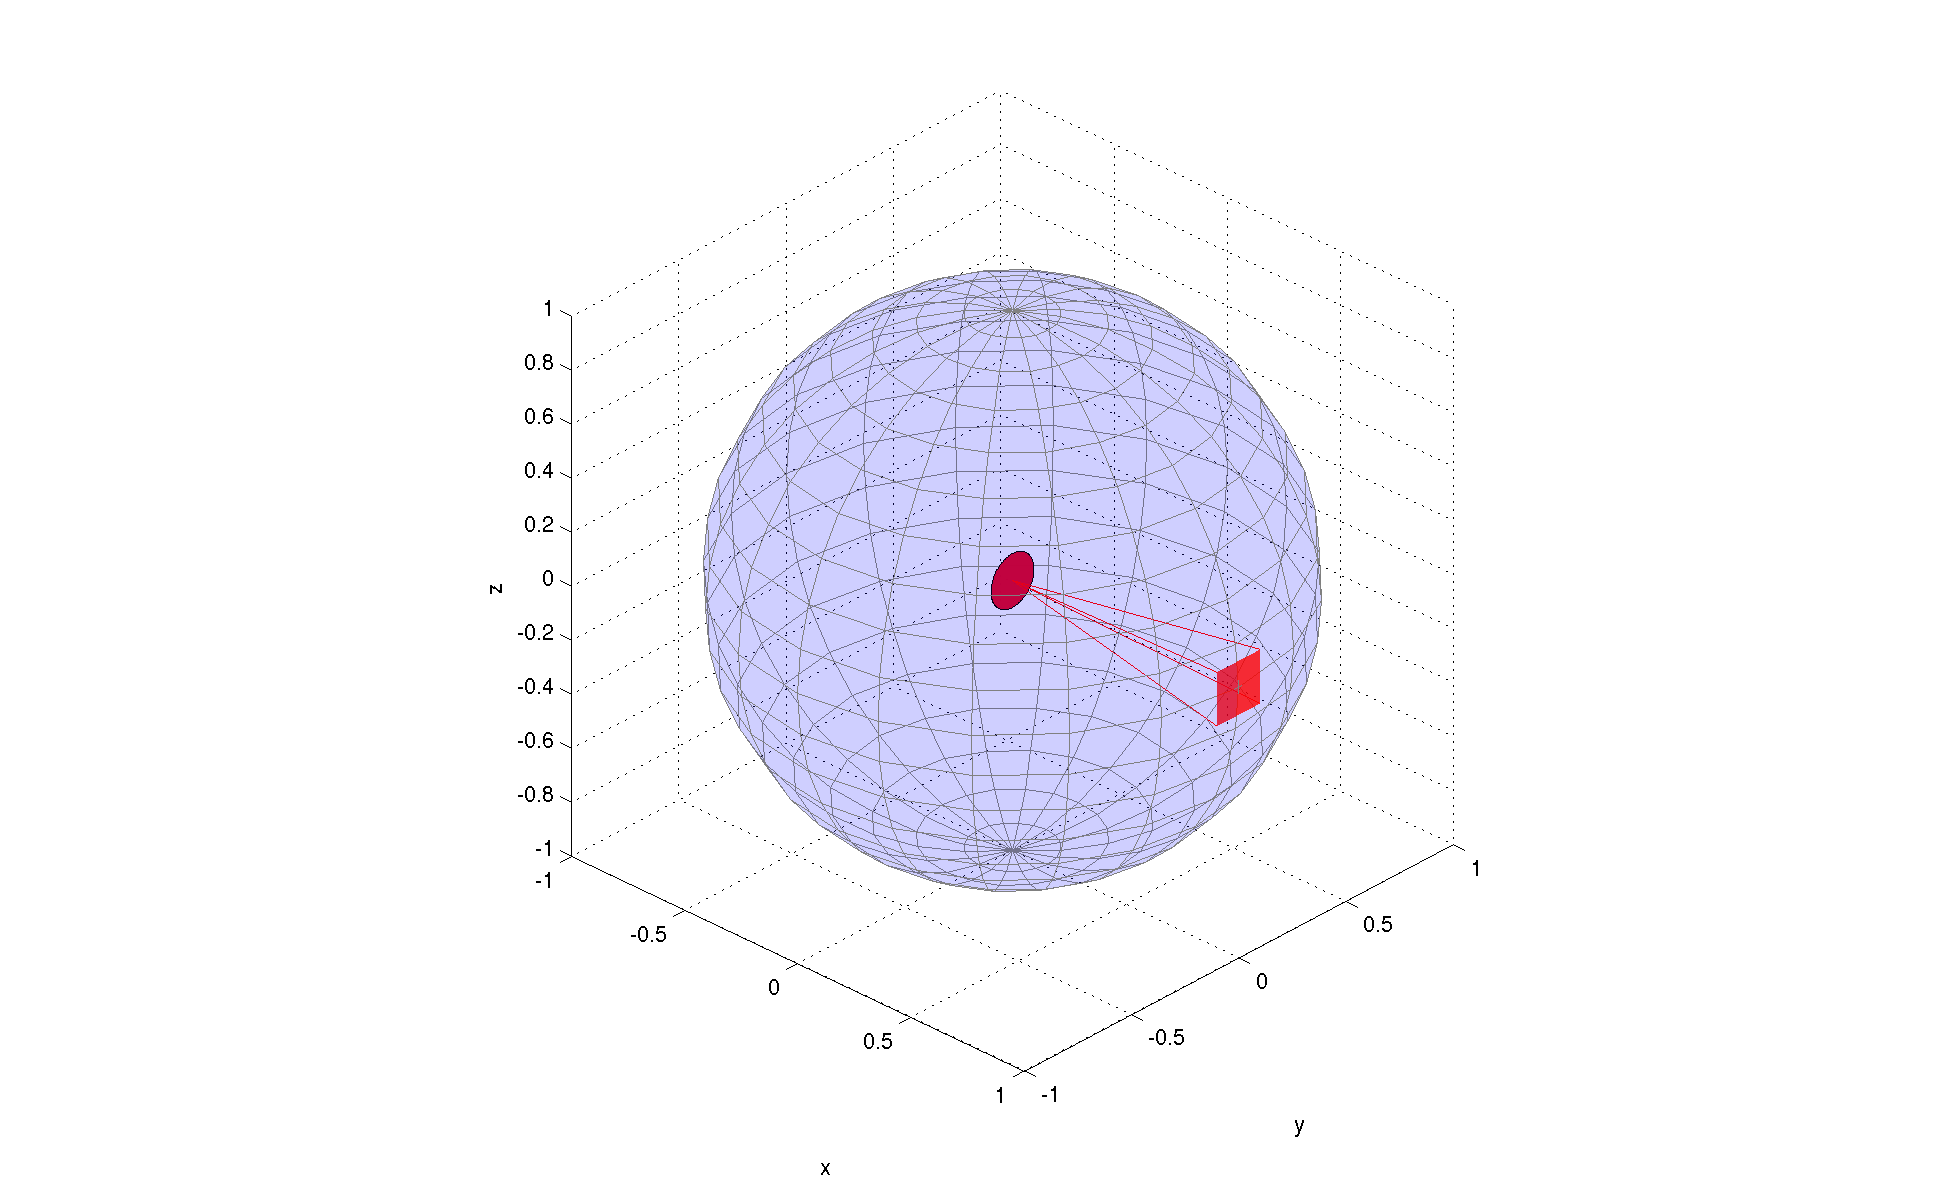
\includegraphics[width=.8\textwidth]{figures/focusing}
\end{center}
\caption{Illustration of the effect of direction focusing in \MCS.
  Weights of neutrons emitted into a certain solid angle are
  scaled down by the full unit sphere area.}
\label{fig:focusing}
\end{figure}

\section{Adaptive and Stratified sampling}
\index{Monte Carlo method!adaptive sampling}
\index{Monte Carlo method!stratified sampling}
\index{Adaptive sampling}
\index{Stratified sampling}
\index{Sampling}
\index{Variance reduction}

Another strategy to improve sampling in simulations
is \emph{adaptive importance sampling} (also called variance reduction technique), % \cite{importance},
where \MCS during the simulations will determine
the most interesting directions and gradually change
the focusing according to that.
Implementation of this idea is
found in the \textbf{Source\_adapt} and \textbf{Source\_Optimizer} components.
%, described in section~\ref{s:Source_adapt}.

An other class of efficiency improvement technique is the so-called \emph{stratified sampling}. It consists in partitioning the event distributions in representative sub-spaces, which are then all sampled individually. The advantage is that we are then sure that each sub-space is well represented in the final integrals. This means that instead of shooting $N$ events, we define $D$ partitions and shoot $r=N/D$ events in each partition. In conjunction with adaptive sampling, we may define partitions so that they represent 'interesting' distributions, e.g. from events scattered on a monochromator or a sample. The sum of partitions should equal the total space integrated by the Monte Carlo method, and each partition must be sampled randomly.

\index{Virtual sources}
In the case of \MCS, an ad-hoc implementation of adaptive stratified is used when repeating events, such as in the Virtual sources (Virtual\_input, Vitess\_input, Virtual\_mcnp\_input, Virtual\_tripoli4\_input) and when using the SPLIT keyword in the TRACE section on instrument descriptions. We emphasize here that the number of repetitions $r$ should not exceed the dimensionality of the Monte Carlo integration space (which is $d=10$ for neutron events) and the dimensionality of the partition spaces, i.e. the number of random generators following the stratified sampling location in the instrument.

\section{Accuracy of Monte Carlo simulations}
\index{Monte Carlo method!accuracy}

When running a Monte Carlo, the meaningful quantities are obtained by integrating random events into a single value (e.g. flux), or onto an histogram grid. The theory \cite{James80} shows that the accuracy of these estimates is a function of the space dimension $d$ and the number of events $N$. For large numbers $N$, the central limit theorem provides an estimate of the relative error as $1/\sqrt{N}$. However, the exact expression depends on the random distributions.

\MCS uses a space with $d=10$ parameters to describe neutrons (position, velocity, spin, time). We show in Table \ref{t:mc_accuracy} a rough estimate of the accuracy on integrals as a function of the number of records reaching the integration point. This stands both for integrated flux, as well as for histogram bins - for which the number of events per bin should be used for $N$.

\begin{table}
  \begin{center}
  {\let\my=\\
    \begin{tabular}{|c|c|}
    \hline
    Records       & Accuracy \\
    \hline
    $10^3$ & 10 \% \\
    $10^4$ & 2.5 \% \\
    $10^5$ & 1 \% \\
    $10^6$ & 0.25 \% \\
    $10^7$ & 0.05 \% \\
    \hline
    \end{tabular}
    \caption{Accuracy estimate as a function of the number of statistical events used to estimate an integral with \MCS.}
    \label{t:mc_accuracy}
  }
  \end{center}
\end{table}

